
\section{Susceptibility calculations}
    \label{Sec:ResD:SubsceptibilityCalculation}

To verify that we do get enhanced susceptibility, which may lead to a spin-density wave state, the $q$-dependant susceptibility -- described in section \ref{Sec:Theo:Susceptibility} -- was calculated. Since the Lindhard function takes the sum over all energies in the \ac{BZ}, there may be some concern that the rather crude adjustments to the \ac{DFT} calculations performed in the previous section -- which have only been verified to be correct for energies at the Fermi surface -- may give erroneous results. However the nature of the Lindhard function means that far greater weight is given to energies that are near the Fermi surface. Figure~\ref{Fig:ResD:ShiftedBandStructure} shows the `spaghetti plot' with the energies tweaked as described in the previous section. We see that there are discontinuities in band 2, most notably between $Z$ and $\Sigma_1$, due to the correction applied proportional to the \DzTwo character, however these are reasonably far from the Fermi level and so shoudl not affect the calculations significantly.
\begin{figure}[htbp]
    \begin{center}
        \includegraphics[scale=0.9]{Chapter-dHvABaFe2P2/Figures/AngleDepMeasurements/ShiftedBandStructure/ShiftedBandStructure}
        \caption{Band structure for the bands that cross the fermi surface shifted to fit the dHvA data. (a) and (b) give an idea of the granularity of the \WIEN calculation at the Fermi surface. Inset shows the path around the \ac{BZ}.}
        \label{Fig:ResD:ShiftedBandStructure}
    \end{center}
\end{figure}

Calculations were performed using the \code{calc_x0.m} code described in section\ref{Sec:Exp:Susceptibility} using a $93\times93\times93$ grid of energy values that covered the first \ac{BZ}. We will need to smooth over the granularity of the \WIEN band model since for the imaginary part at least, the calculation is very sensitive to slight imperfections in cancellation near the Fermi energy. Referring to figure~\ref{Fig:ResD:ShiftedBandStructure}, there are two regions in the marked (a) and (b) which show points around the Fermi level as they are spaced in the $93\times93\times93$ model. (a) is particularly steep and has a $\Delta \epsilon/\Delta\textrm{pt.} = \unit{0.0760}{\electronvolt}$ and (b) is more typical of the gradient at the Fermi level and has $\Delta \epsilon/\Delta\textrm{pt.} = \unit{0.0368}{\electronvolt}$. So the energy scale that will need to compensated is $\sim$\unit{2-5\ten{-3}}{Ry}.

\begin{figure}[htbp]
    \begin{center}
        \includegraphics[scale=0.9]{Chapter-dHvABaFe2P2/Figures/Susceptibility/RangeDeltaOmega/RangeDeltaOmega}
        \caption{Qualitative plots of the real and imaginary part of the Lindhard susceptibility calculated at $k_z=\pi$ for $T=\unit{157}{\kelvin}$ and a range of $\delta$ and $\omega$ values.}
        \label{Fig:ResD:RangeDeltaOmega}
    \end{center}
\end{figure}

Susceptibility was calculated for a wide range of magnitudes of $\delta$ and $\omega$ in order to guage qualitative behaviour with the resulting plots shown in figure~\ref{Fig:ResD:RangeDeltaOmega}. Both the real and imaginary parts undergo qualitative changes as the parameters are adjusted above the spacing corresponding to the typical gap in energy between points. The imaginary part also undergoes a qualitative change when $\omega$ falls below \unit{1\ten{-5}}{Ry} and there is also an increase in noise when $\delta$ falls below a similar energy threshold. We continue using $\delta=1\ten{-3}$ and $\omega=1\ten{-3}$ which correspond approximately the the energy scale of the spacing as well as the energy scale of the temperature smearing.

\begin{figure}[htbp]
    \begin{center}
        \includegraphics[scale=0.9]{Chapter-dHvABaFe2P2/Figures/Susceptibility/2DSusceptibility/2DSusceptibilityPlusAltKz}
        \caption{Real and imaginary part of the Lindhard susceptibility are plotted on the left and right respectively. Upper panels are at $k_z=\pi$ and lower are at $k_z=0$. For these calcualtions $\delta=1\ten{-3}$, $\omega=1\ten{-3}$ and $T=\unit{157.88}{\kelvin}$. Insets show contour plots for the respective surface plots.}
        \label{Fig:ResD:2DSusceptibility}
    \end{center}
\end{figure}
The upper panel of figure~\ref{Fig:ResD:2DSusceptibility} shows the quantified plots for the real and imaginary parts of the susceptibility at the chosen values of $\delta$ and $\omega$. The contour plots in the insets show the two-fold symmetry due to the choice of $k_z=\pi$. Unlike LaFeAsOF where the two dimensional approximation is a good one, this is not necessarily the case for \BaFeP which features a strongly three-dimensional hole band and some warping of the electron bands. The lower panels present the same calculation performed at $k_z=0$ which shows little change other than a rotation of the susceptibility bias due to the screw symmetry of the electron bands.

\begin{figure}[htbp]
    \begin{center}
        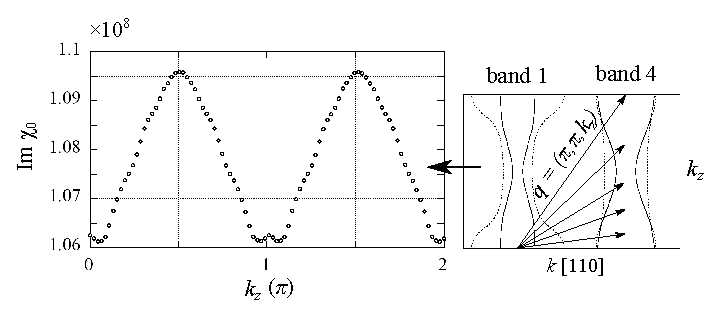
\includegraphics[scale=0.7]{Chapter-dHvABaFe2P2/Figures/Susceptibility/NestingVector/NestingVector}
        \caption{Left panel shows the imaginary part of the Lindhard susceptibility between bands summed with their reciprocals for $q=(\pi, \pi, k_z)$ over the height of the \ac{BZ}. We see enhancements at $k_z=\pi/2,3\pi/2$ for bands 1-4 and 2-3 and at $k_z=0,\pi,2\pi$ for bands 2-3 and 2-4.}
        \label{Fig:ResD:NestingVector}
    \end{center}
\end{figure}
To verify that there is indeed a nesting conditions at some $k_z$ for $q=(\pi, \pi, k_z)$ figure~\ref{Fig:ResD:NestingVector} presents the imaginary part of the susceptibility vs. $k_z$ for a range of nesting vectors. Each coupling of bands is summed both ways --- e.g. 4-1 is summed with 1-4 --- and plotted in order ot obtain the residual difference due to $\omega$. Unsurprisingly, we see that self coupling results in very little weight with hole-hole and electron-electron coupling also resulting in little weight. The strongest component is due to bands 2-4 which also demonstrates a strong enhancement of around $25\%$ at $k_z=0,\pi,2\pi$. Band 2 also couples strongly with band three at the same $q$ vectors with around a $17\%$ enhancement. Band 1 couples strongly with band 4 but at $k_z=\pi/2,3\pi/2$ with the largest enhancement of around $38\%$. Band 1 also couples less strongly with band $3$ at the same $k_z$ with an enhancement of around $15\%$. The total susceptibility is determined mostly by the coupling of band 2 but only has a relatively moderate enhancement of around $7.4\%$ at $kz=0,\pi,2\pi$.

Figure~\ref{Fig:ResD:ZSlices} shows cross sections of the final corrected Fermi surfaces showing the basal-plane at the bottom of the unit cell ($k_z=0$), quarter of the way up, ($k_z=0.25$) and halfway up ($k_z=0.5$). The inner hole surface (band 1) at $k_z=0.5$ directly matches the size and shape of the inner electron surface (band 4) at $k_z=0.25$ which is the likely cause of the strong enhancement observed in the susceptibility. Moreover, the bands share similar predominant \DxzDyz orbital character. The strong enhancements between bands 2 and 4 are also shown in the figure as a dashed arrow.

\begin{figure}[htbp]
    \begin{center}
        \includegraphics[scale=0.9]{Chapter-dHvABaFe2P2/Figures/AngleDepMeasurements/ZSlices/ZSlices}
        \caption{Cross sections of the corrected Fermi surface in the $ab$ plane (panels 1, 2 and 3) and in the $[110]$ plane (panel 4). Markings correspond to the orbital character of the Fermi surface slices. Two nesting vectors are shown as long arrows.}
        \label{Fig:ResD:ZSlices}
    \end{center}
\end{figure}

These enhancements at $q=(\pi, \pi)$ show that partial nesting does indeed occur in this material demonstrating that this condition alone is not sufficient for superconductivity to occur. This concludes the Fermiology results, we now move onto the mass enhancements.

